\section{Instantaneous Energetic Cost}
The instantaneous energetic cost, our objective function, is estimated through continuous breath measurements over a lengthy duration of time. \citet{Brockway1987} developed a formula for converting $CO_2$ and $O_2$ measurements into a metabolic cost, which is then fit into a first-order dynamical model. Given the noisiness of respiratory measurements, previous studies \citep{Felt2015,Selinger2014} allowed three minutes while subjects reached a steady state before measuring for an additional three minutes to estimate an instantaneous energetic cost. In a previous Bayesian optimization study \citep{Ding2018}, each iteration used a fixed two minutes of respiratory measurements. 

Rather than requiring a fixed time interval for each evaluation, we aim to ascertain an accurate estimate only for promising parameter settings while stopping early for those that are unlikely to improve upon the best settings found so far. To make that determination, an online estimator for instantaneous energetic cost was developed using the metabolic cost model
\begin{align}
m_t(c_0, c, \tau_0, \tau) = c(1-e^{\frac{-t}{\tau}}) + c_0e^{\frac{-t}{\tau_0}},
\end{align}
where $t$ is the total measurement time in seconds and $\tau_0, \tau$ are time constants characterizing the rate of change for the initial cost $c_0$ and the instantaneous energetic cost $c$ respectively.

\begin{figure}[t]
\centering
\includegraphics[width=\textwidth]{metabolicestimation.png}
\caption{Sample estimation process for instantaneous energetic cost.}
\label{fig:metabolicestimation}
\end{figure}

\section{Parameter Estimation}
The time and cost parameters are estimated through an Unscented Kalman Filter \citep{julier1997}. Kalman filters are applied to discrete time systems of the form
\begin{align}\begin{split}
  x(t+1) &= F(x(t), v(t), t)\\
  z(t) &= H(x(t), w(t), t),
\end{split}\end{align}
where $x(t)$ represents the unobserved state of the system, $z(t)$ the observed measurement, and zero-mean Gaussian vectors $v(t)$ for process disturbances or modeling errors and $w(t)$ for measurement noise. 

First, a prediction is made for the state of the system after one timestep. Let $\hat{x}(t\vert t-1)$ represent the estimate for $x(t)$ using measurements $\mathbb{Z}(t-1)=[z(1), z(2), ..., z(t-1)]$ and $P_{x}(t\vert t-1)$ the covariance for the estimate. The prediction step aims to calculate
\begin{align}\begin{split}
  \hat{x}(t\vert t-1) &= \mathbb{E}[F(x(t-1), v(t-1), t-1)\vert \mathbb{Z}(t-1)]\\
  P_{x}(t\vert t-1) &= \mathbb{E}[\{ \hat{x}(t\vert t-1) - x(t) \} \{ \hat{x}(t\vert t-1) - x(t) \}^T \vert \mathbb{Z}(t-1)].
\end{split}\end{align}

The prediction is then reconciled with the observed measurement through a minimum mean-squared estimate $\hat{x}(t)$ and covariance $P_{x}(t)$ according to the following equations
\begin{align}
\begin{split}
  \hat{x}(t) &= \hat{x}(t\vert t-1) + Ky \\
  P_{x}(t) &= P_{x}(t\vert t-1) - KP_{y}(t\vert t-1) K^T\\
  K &= P_{xy}(t\vert t-1) P_{y}^{-1}(t\vert t-1)\\
  y &= z(t) - H(\hat{x}(t\vert t-1) , w(t), t).
\end{split}
\end{align}

The underlying requirement for these equations is an accurate propagation of the first two moments of $x(t)$ and $z(t)$. As such, Gaussian estimates are used as they assume the least information. When $F$ or $H$ is nonlinear, rather than linearizing the functions with a first order approximation the UKF approximates its probability distribution through an unscented transformation. The complete implementation details are outlined in Appendix \ref{ch:append-ukf}.

As we consider $\tau_0, \tau, c, c_0$ to be constant parameters, our UKF setup is
\begin{align}
\begin{split}
  x &= [c_0 \text{ } c \text{ } \tau_0 \text{ } \tau]\\
  F(x(t), v(t), t) &= x(t) + v(t)\\
  H(x(t), w(t), t) &= m_t(x(t)) + w(t).
\end{split}
\end{align}

\section{UKF Covariance Parameters}\label{sec:ukfcovar}
The UKF algorithm has covariance parameters $P_{x}$ for the state estimate, $P_{w}$ for measurement noise, and $P_{v}$ for process noise that determine the sensitivity of the state estimate to new measurements. Table \ref{tab:esttuningparams} summarizes the effect of increasing one of these covariance parameters while holding all others constant.

\begin{table}[h]
  \centering
  \begin{tabular}{ | c | M{10cm} |}
  \hline
  &\\
  Increase & Effect On State Estimate \\ 
  &\\
  \hline
  &\\
  $P_x$ & A higher initial covariance on the state estimate implies higher uncertainty with the state prior. Early observations will have a greater effect on the state update. However, $P_x$ decreases after every state update; observations therefore will have a smaller effect on the state estimate over time\\ 
  &\\
  \hline
  &\\
  $P_w$ & A higher measurement noise will reduce an observation's effect on the state update. The state will be slow to move away from the prior, particularly in early observations. $P_w$ also affects $P_x$ on future timesteps, as it is bounded by $P_w$\\ 
  &\\
  \hline
  &\\
  $P_v$ & While $F$ is essentially the identity function in the metabolics model as the cost and time parameters are assumed to be constant, $P_v$ encapsulates the error in that model as well as outside disturbances that can't be measured such as fatigue. Increasing $P_v$ can be used to enforce a lower bound on the effect of an observation to the state update\\ 
  &\\
  \hline

  \end{tabular}
  \caption{Tuning Parameters for metabolic estimator}
  \label{tab:esttuningparams}
\end{table}

The volatility of the estimator is dependent on the calibration of the covariance parameters with respect to the noise of the measurements. Figure \ref{fig:measurementnoise} shows three estimators: one that underestimates the measurement noise by a factor of 10, one that is exact, and one that overestimates by a factor of 10. Underestimating leads to a higher weight given to the measurement on subsequent state updates, with the volatility initially quite high. As more measurements are taken and $P_x$ decreases, the estimator eventually reaches a steady state. On the other hand, assuming too high a measurement noise will cause the estimator to slowly update towards the true value.

\begin{figure}[t]
\centering
\includegraphics[width=\textwidth]{measurementnoise.png}
\caption{With a true instantaneous energetic cost at 350 and and prior at 300, keeping all other parameters constant, the effect of using various $P_w$ values on measurement variance.}
\label{fig:measurementnoise}
\end{figure}

\section{Initial Trials and Future Work}
Using previously attained metabolic data, Figure \ref{fig:ukftuned} shows the raw and noisy measurements taken and the metabolic cost prediction that the model developed in response to a representative participant\footnote{Testing carried out by Myunghee Kim}. The bottom plot displays the covariance associated with the cost, beginning with a covariance of 1 and converging at different rates depending upon the raw data. When tuned properly, both trials see a relatively smooth rate of convergence of the estimate. With varying amounts of data provided, the accuracy in percent error was calculated by comparing with a "ground truth" value at each termination condition (5 min, 2 min, 1.5 min, 20 breaths, and 30 breaths). This ground truth value is the average of the last two minutes of data, when the subject has reached steady-state.

\begin{figure}[!ht]
\centering
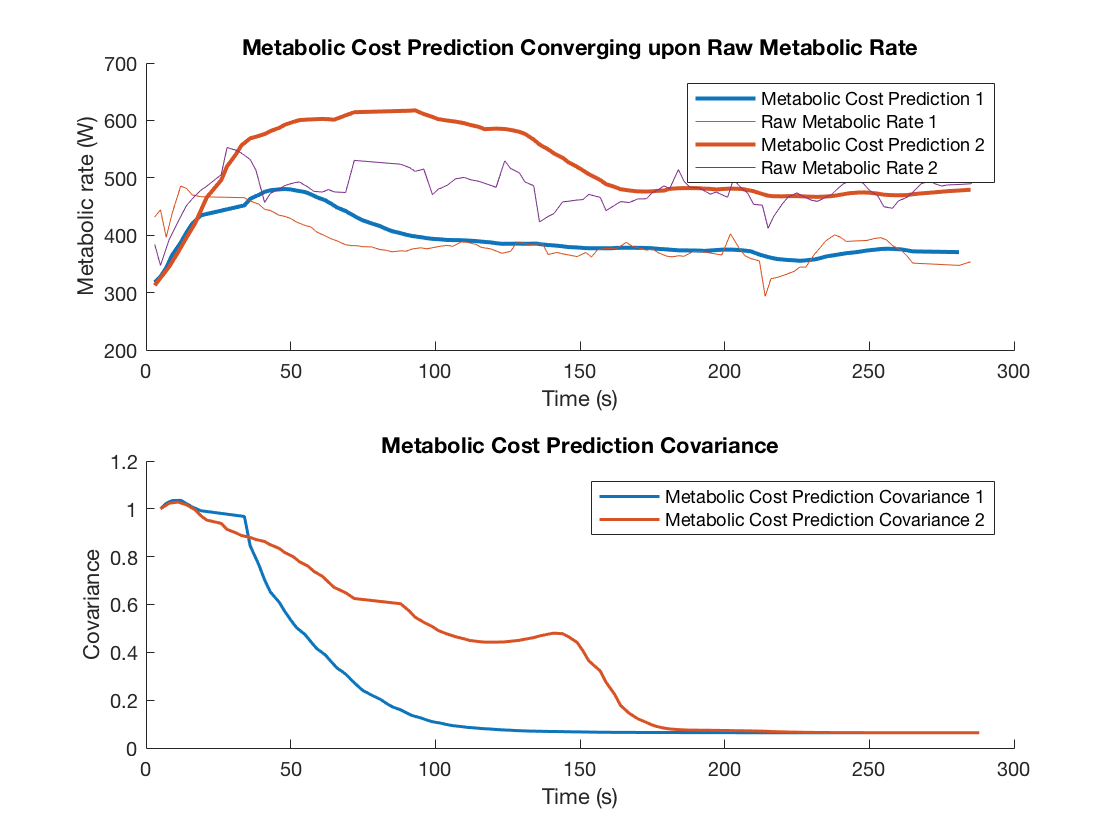
\includegraphics[width=\textwidth]{ukf}

\begin{tabular}{ |c|c|c| } 
 \hline
 Data Used & Average $R^2$ & Max \% Error \\ 
 \hline
 Full Trial & 0.996 & 0.977\% \\ 
 2 Minutes & 0.984 & 0.984\% \\ 
 1.5 Minutes & 0.973 & 0.973\% \\ 
 30 Breaths & 0.966 & 3.113\% \\ 
 20 Breaths & 0.890 & 5.767\% \\ 
 \hline
\end{tabular}%
%}
\caption{Tuned UKF Estimator over previously collected data. Accuracy assessed over partial data.}
\label{fig:ukftuned}
\end{figure}

During trial testing for our optimization methods, the same noise covariances used on the UKF estimator showed various levels of volatility across subjects (Figure \ref{fig:subjcostest}). This suggests the estimator should also have some subject-to-subject individualization based on the volatility of respiratory measurements. Future work would involve creating a cost function to optimize for this variation, balancing between the smoothness of the estimation curve and eventual convergence to the "true" instantaneous energetic cost. As Bayesian optimization starts with an exploration phase, the estimator can then be tuned a posteriori. Depending on the speed of the optimization, the estimator could potentially be tuned after every evaluation that takes the full duration, making it adaptable over time to external factors such as fatigue. Improvements in tuning the estimator would have residual effects in the information provided to both the Gaussian process and the stopping problem. Without it, Chapter \ref{ch:3} will introduce the stopping problem and different models that take into account the accuracy of the estimator. 

\begin{figure}[t]
\centering

\includegraphics[width=\textwidth]{subjcostest.png}
\caption{Tuned UKF Estimator shows different levels of volatility during optimization studies on different subjects.}
\label{fig:subjcostest}
\end{figure}